\chapter{Kajian Pustaka}

\section{Premature Ventricular Contractions (PVCs)}
Aktivitas denyut jantung yang terjadi pada manusia adalah disebabkan terjadinya aktivitas elektrik jantung yang dilakukan oleh SA-Node dan AV-node\cite{heart_act}. SA-node atau Sino-Atrial Node adalah bagian kecil dari jaringan jantung yang terdapat di bagian atrial dan berfungsi untuk melakukan pelepasan electron yang kemudian akan memacu atrial berkontraksi. Selanjutnya elektron yang dilepaskan oleh SA-node akan ditangkap oleh AV-node melalui jaringan-jaringan kecil di jantung yang kemudian akan dilepaskan kembali oleh AV-node sehingga membuat bagian ventrikel jantung bekontraksi \cite{khandait2012}. Aktifitas-aktifitas pelepasan elektron yang dilakukan oleh SA-node dan AV-node ini lah yang kemudian membuat jantung berdenyut secara ritmik dan teratur. PVC adalah salah satu kelainan jantung yang disebabkan karena ketidaknormalan denyut jantung. Pada PVC, ventrikel berkontraksi secara prematur atau melepaskan elektron sebelum menerima elektron yang dikirimkan oleh SA-node\cite{Kanwar2015}.

\section{Feature Extractions}
\textit{Feature extraction} adalah tahap awal yang dilakukan pada proses deteksi kelainan jantung setelah tahap pre-prosessing pada sinyal EKG. Tahap \textit{feature extraction} ini bertujuan untuk mendapatkan titik P, QRS,T dan nilai-nilai penting lainnya pada gelombang EKG. Nilai-nilai gelombang ini kemudian akan menjadi nilai masukan pada tahap klasifikasi dan dilakukan analisis terhadap nilai-nilai gelombang tersebut. Tingkat akurasi yang dihasilkan pada tahap \textit{feature extraction} cukup menentukan nilai akurasi akhir pada keseluruhan proses deteksi PVC\cite{Huang2015Thesis}. Selain itu \textit{feature extraction} yang baik juga akan membuat proses diagnosa menjadi lebih efisien\cite{Karpagachelvi2010,Chang1987,UMaji}. Karena itu menggunakan algoritma yang sederhana namun tetap mempertahankan akurasi yang optimal dalam tahap \textit{feature extraction} menjadi sangat penting.

\section{Riset Deteksi PVC}
Tahun 1987, Chang\cite{Chang1987} telah mengusulkan sebuah algoritma \textit{feature extraction} yang dapat digunakan secara real-time dan berbasis \textit{microprocessor}. Setelah diujikan kepada 18 orang pasien metode ini mencapai nilai akurasi sebesar 99,3 persen dan sensitivitas 81,12 persen.

Selanjutnya pada tahun 2012, A.Ouelli et al\cite{A.Ouelli2012_AR} menggunakan AR modeling dan algoritma Multi Layer Perceptron untuk membuat metode deteksi arrythmia. Tujuan Ouelli dalam mengajukan metode ini adalah untuk membuktikan bahwa algoritma AR (\textit{Autoregressive} Modeling) memiliki kemampuan untuk menghasilkan hasil \textit{feature extraction} yang sangat baik. Hasil akurasi yang diperoleh Ouelli dengan menggunakan AR modeling dan MLP ini mencapai angka 99,6 persen.

Di tahun yang sama Chen\cite{RobertChen} juga mengusulkan algoritma baru untuk melakukan deteksi PVC secara real-time berbasis Wavelet Transform. Sistem deteksi PVC yang diajukan memiliki dua bagian proses, yaitu proses deteksi puncak R dan proses deteksi sinyal PVC. Algoritma \textit{feature ectraction} yang digunakan adalah algoritma Mallat dan Lipschitz exponent untuk mendapatkan puncak R dan metode \textit{sum of trough} untuk deteksi PVC. Pada saat deteksi PVC digunakan juga RR-interval sebagai nilai threshold. Hasil penelitian ini menghasilkan akurasi sebesar 94,73 persen.

U Maji \cite{UMaji} dalam jurnalnya di tahun 2013 mencoba melakukan metode deteksi AF/Atrial Fibrillation menggunakan Empirical Mode Decomposition dan pendekatan secara statistik. EMD adalah metode dekomposisi sinyal yang telah banyak diterapkan dalam menganalisis morfologi dari sinyal non-stationer seperti ECG. Tahap pertama yang dilakukan adalah melakukan dekomposisi sinyal yang telah dilakukan denoising ke dalam fungsi IMF (Intrinsic Mode Function) kemudian diberikan parameter varian dan standar deviasi untuk melakukan klasifikasi dari setiap data IMF yang ada. Meskipun algoritma EMD ini baru pertama kali diterapka untuk mendeteksi AF, tetapi sudah mampu memiliki nilai \textit{sensitivity} dan \textit{specificity} sebesar 96 persen dan 93 persen. EMD juga termasuk algoritma yang adaptive dan sangat efisien \cite{UMaji}.

Fahruzi \cite{fahruzi} dalam jurnalnya melakukan percobaan deteksi PVC menggunakan kombinas \textit{RR Interval} dan \textit{coeeficient Correlation} untuk mengekstrak informasi penting dari ECG. Pengujian dilakukan dalam rentang waktu data 1 menit yang mewakili bentuk gelombang normal dan gelombang PVC. Percobaan ini menghasilkan akurasi sebesar 99,93 persen dan sensitivitas 97,06 persen. 

Deteksi Arryhthmia juga dilakukan oleh \cite{rameshwari} dengan menggunakan algoritma Pan-Tomkins untuk mendeteksi R peak. \cite{rameshwari} mengatakan bahwa efektifitas deteksi yang dilakukan bergantung dari hasil ekstraksi titik P-Q-R-S dan T yang benar. Pada deteksi PVC yang dilakukan memperoleh sensitivitas sebesar 96,15 persen dan spesifikasi sebesar 92,59 persen.   

\cite{Arief2015} berhasil membuat sistem deteksi PVC pada perangkat Android. Ekstraksi fitur yang dilakukan menggunakan software Android Java eclipse Juno untuk mendapatkan interval RR dan lebar QRS. Kemudian tahap klasifikasi dilakukan dengan algoritma ANN menggunakan software MATLAB. Eksperimen yang dilakukan ini tidak menyebutkan secara jelas algoritma apa yang digunakan dalam ekstraksi fitur. Hasil eksperimen ini memiliki nilai akurasi 96,2 persen, 	spesifikasi 96,58 persen dan sensitivitas 94,58 persen.

Sistem deteksi PVC berbasis mobile lainnya juga dilakukan oleh Pedro\cite{Pedro2014}. Pedro membangun algoritma tersendiri untuk mendeteksi RR interval dan \textit{linear classifier design}. Algoritma ini menghasilkan nilai sensitivitas 90,13 persen dan spesifikasi 82,52 persen.

Huang et al \cite{Huang2015Thesis} pada tahun 2015 juga menggunakan wavelet transform tetapi tanpa menggunakan AR modeling. Dengan classifier yang sama seperti yang dilakukan oleh Zhao yaitu SVM Huang mendapatkan nilai akurasi 93,17 (persen) Melalui thesis miliknya ini akhirnya Huang mengambil kesimpulan bahwa karakteristik gelombang EKG yang dikirimkan kepada classifier sangat menentukan nilai akurasi akhir dari classifier tersebut. 

Lek-Uthai \cite{Lekuthai2014} menggunakan 3 tahap prosedur dalam ektraksi fiturnya yaitu, deteksi QRS complex, \textit{smoothing} untuk mengeliminasi \textit{high frequency} pada gelombang EKG sebelum melakukan ekstraksi bentuk QRS menjadi interval QRS, dan menghilangkan \textit{baseline}. Fitur yang diambil dari gelombang adalah interval RR, bentuk QRS, lebar QRS dan ketinggian ST (ST-level). Hasil dari uji coba ini menghasilkan sensitivitas 99,47 persen dan spesifiksai 99l24 persen. Classifier yang digunakan adalah \textit{binary classification}.

Perbandingan hasil penelitian di atas dapat dilihat pada tabel di bawah ini : 
\begin{figure}[h!]
	\centering
	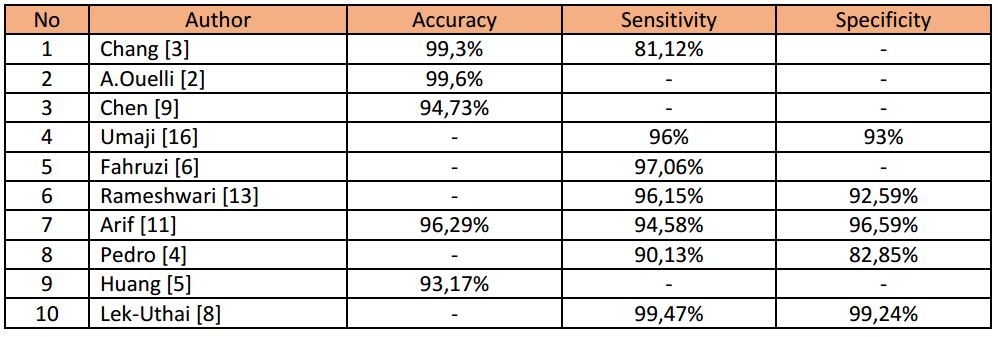
\includegraphics[scale=0.5]{comparison-tab.png}
	\caption{Tabel Perbandingan Hasil Riset}
	\label{fig:my_auth}
\end{figure}
